\documentclass[12pt]{report}
\usepackage{graphicx} % Required for inserting images
\usepackage[a4paper, margin=2.5cm]{geometry}
\graphicspath{{../.images/}}

\title{CMP6200 Individual Undergraduate Project}
\author{Lewis Higgins - Student ID 22133848}


\usepackage[utf8]{inputenc}
\usepackage[T1]{fontenc}
\usepackage{float} % here for H placement parameter
\usepackage{subcaption}

\usepackage{filecontents}
\usepackage[
    firstinits=true, % render first and middle names as initials
    useprefix=true,
    maxcitenames=3,
    maxbibnames=99,
    style=authoryear,
    dashed=false, % re-print recurring author names in bibliography
    natbib=true,
    url=false,
    sorting=none
]{biblatex} % biblatex config for harvard refs

\renewbibmacro*{volume+number+eid}{%
    \printfield{volume}%
%  \setunit*{\adddot}% DELETED
    \setunit*{\addnbspace}% NEW (optional); there's also \addnbthinspace
    \printfield{number}%
    \setunit{\addcomma\space}%
    \printfield{eid}}
\DeclareFieldFormat[article]{number}{\mkbibparens{#1}}

\DeclareLabeldate{\field{date}\field{eventdate} \field{origdate}\literal{nodate}}

\addbibresource{proposal.bib}

% Use single quotes around titles:
\usepackage[british]{babel}
\usepackage{csquotes}

\usepackage{hyperref}

\hypersetup{
    colorlinks=true,
    linkcolor=black,
    filecolor=magenta,
    urlcolor=blue,
    citecolor=black,
}


\urlstyle{same}


% To prevent "Chapter N" display for each chapter
\usepackage[compact]{titlesec}
\usepackage{wasysym}
\usepackage{import}

\titlespacing*{\chapter}{0pt}{-2cm}{0.5cm}
\titleformat{\chapter}[display]
{\normalfont\bfseries}{}{0pt}{\Huge}

\newcommand\blfootnote[1]{
    \begingroup
    \renewcommand\thefootnote{}\footnote{#1}
    \addtocounter{footnote}{-1}
    \endgroup
}


%\lhead{Lewis Higgins - ID 22133848~~~~~~~~~~~~~~~\includegraphics[width=1.75cm]{bcu logo}}
%\fancyhead[R]{\leftmark}

\usepackage{xcolor} % Might be useful

\usepackage{colortbl}
\usepackage{longtable}
\usepackage{amssymb}

\usepackage{pdflscape}

\begin{document}

    \makeatletter
    \begin{titlepage}
        
\includegraphics[width=0.3\linewidth]{BCUWide.jpg}\\[4ex]
        \vspace{1cm}
        \begin{center}
            {\huge \bfseries  CMP6200}\\[2ex]
            {\huge \bfseries  Individual Undergraduate Project}\\[2ex]
            {\huge \bfseries 2024 - 2025}\\[6ex]
            {\large \bfseries A1 - Proposal}\\[10ex]
            {\huge \bfseries University Artifically Intelligent Assistant}\\[6ex]
            
\includegraphics[width=0.1\linewidth]{Symbol.png}\\[40ex]
            Course: Computer \& Data Science\\
            Student Name: Lewis Higgins\\
            Student Number: 22133848\\
            Supervisor Name: Dr. Atif Azad
        \end{center}
    \end{titlepage}
    \makeatother
    \thispagestyle{empty}
    \newpage

    \tableofcontents
    %\footnotesize{\listoffigures}

    \chapter{Introduction}\label{ch:introduction}
    \section{Background and Rationale}
    With artificial intelligence (AI) becoming increasingly more powerful and useful in 
    recent years, in some cases even surpassing humans in areas like language and image 
    recognition~\autocite{owid-artificial-intelligence}. It is therefore essential that 
    higher education institutions take advantage of it and ensure to keep up-to-date with its
    developments in the interest of academic integrity, which was also stated in the 
    Higher Education Policy Report dated 28 March 2024 - "Higher education will have to adopt,
    adapt, collaborate and lead to take advantage of AI while managing the risks"~\autocite{AIUni}.\\
    
    \noindent This project aims to leverage recent technical developments in natural language processing (NLP)
    to create a digital assistant for university life that students can use to gain information on topics
    such as university policies and locations on campus. This is because attending university for the first time
    is a daunting and stressful experience for many, often due to it being a new and unfamiliar environment 
    where students have full independence unlike their previous educational settings, which could possibly 
    lead to declines in academic performance and social activity. Some students may not 
    wish to speak with newer people who they don't know about university topics for fear of 
    ridicule or embarrassment, and would benefit from a digital companion to help them to become 
    acquainted with their new environment without the perceived risk of social judgement.\\

    \noindent Chatbots are also a significant tool across the tech sphere, with 73\% of surveyed web users expecting
    companies to have chatbots for convenient interactions \autocite{chatbotStats}. By giving students a 
    quick and easy tool to get the information they need, they can instead shift their focus to their studies
    instead of being distracted by smaller issues.

    

    \section{Key Themes/Topics}
    This project undertakes the following key themes:

    \begin{itemize}
        \item Natural Language Processing (NLP) 
            \begin{itemize}
                \item As the backbone of this project, extensive research into this topic will be necessary 
                to ensure users have a smooth experience.
            \end{itemize}
        \item Large Language Models (LLMs)
            \begin{itemize}
                \item The final product will be utilising a trained LLM for its backend calculations
                for what to display to the user. It is therefore essential that considerable study 
                is taken into how LLMs function from both a developer and user perspective.
            \end{itemize}
        \item Human-computer interactions
            \begin{itemize}
                \item The interactions between users and chatbots will require meticulous study to ensure
                my project can perform as expected.
            \end{itemize}
        \item Ethics in AI
        \begin{itemize}
            \item Given that the chatbot will be engaging in two-way conversation with end-users, it will
            be important that an ethical standard is maintained.
        \end{itemize}
    \end{itemize}

    \chapter{Aims and Objectives}
    \section{Project Aim}
    This project aims to aid new and existing students alike while they are attending university with 
    helpful information about the university itself, such as university societies, locations/campuses, 
    and policies through the medium of a digital chatbot companion.

    \section{Project Objectives}
    \begin{itemize}
        \item Develop a chatbot capable of accurately answering user queries related to university 
        buildings, policies, and clubs with a 95\% accuracy rate.
        \item Conduct a thorough literature review on AI and Natural Language Processing.
        \item Document all stages of development, highlighting challenges faced during the process.
        \item Manage time effectively to ensure all project milestones are met on a consistent and regular timeframe.
        \item Evaluate the effectiveness of an AI assistant on university student acclimatization.
    \end{itemize}


    \chapter{Project Planning}
    \section{Initial Project Plan}
    \begin{enumerate}
        \item Research
        \begin{enumerate}
            \item Conduct heavy research into machine learning and natural language processing to bolster my 
            knowledge of the topics to assist in the development of the chatbot.
            \item Identify similar projects that already exist to understand where challenges may arise in 
            development and how to differentiate my work to make it stand out and provide unique value.
        \end{enumerate}

        \item Data collection
        \begin{enumerate}
            \item To present users with information from the university, I must first collect this information
            for myself from sources such as the university website and the Student Union.
            \item It will also be useful to survey various students for their perspectives on this project, and 
            how useful it would be to them, as they are the target audience.
        \end{enumerate}

        \item Development of a prototype
        \begin{enumerate}
            \item A prototype of the chatbot could be very useful in demonstrating the potential of this project,
            even before its completion.
            \item This prototype could be distributed as part of a survey of users.
        \end{enumerate}

        \item Evaluation
        \begin{enumerate}
            \item It will be important to identify how smooth the process of development was, and how the final
            product compared to its original expectations. Within the evaluation, any challenges faced along the way,
            as well as how they were overcome during development, should be documented in the interests of further
            research.
        \end{enumerate}

        \item Finalisation and submission
        \begin{enumerate}
            \item At the very end of the process, when the chatbot and documentation are in acceptable states,
            final changes will be made based on supervisor and user feedback before making the final submission.
        \end{enumerate}
    \end{enumerate}

    \vspace{0.5cm}
    \noindent Below is a Gantt chart documenting an early concept of the development timeline throughout the year.

    \pagebreak

    \begin{landscape}

    \begin{figure}[H]
        \centering
        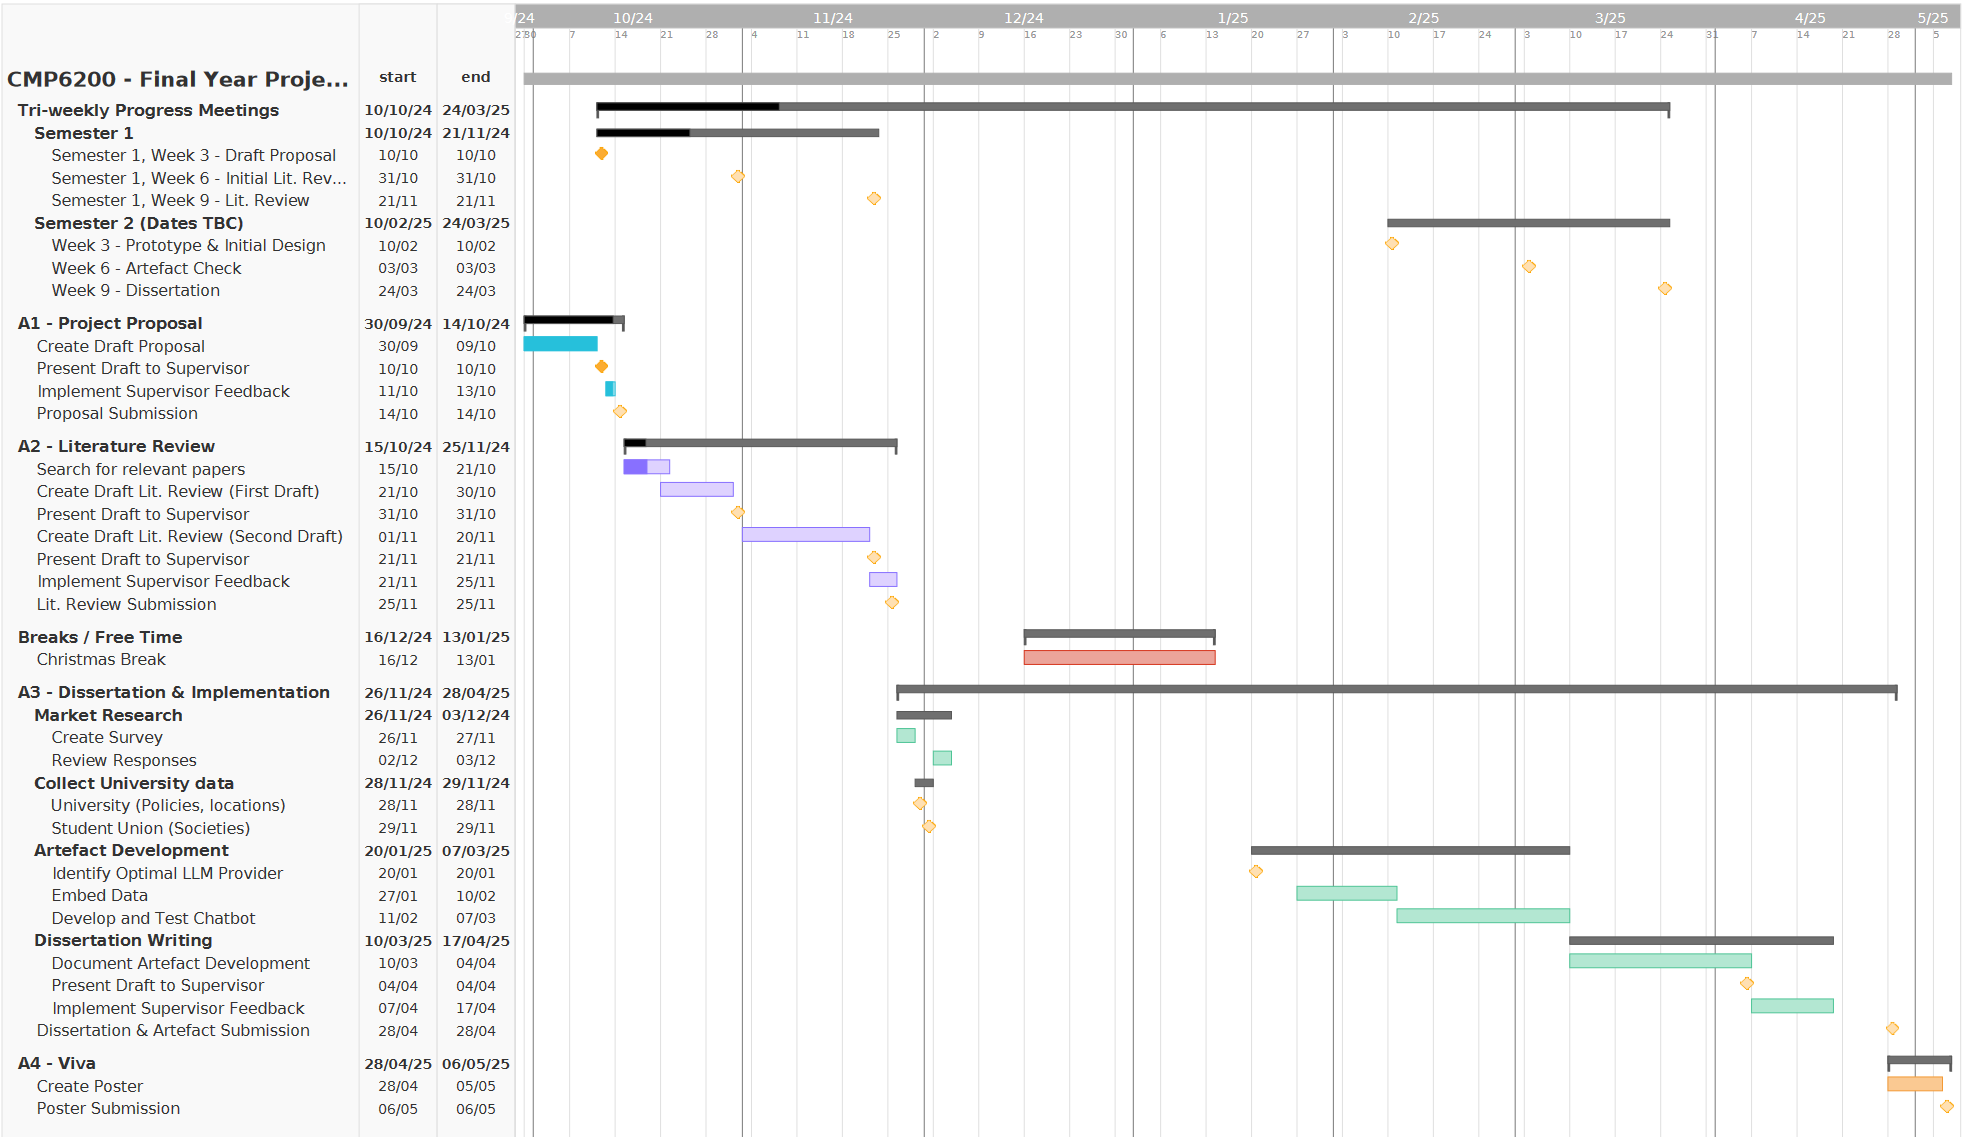
\includegraphics[width=.9\linewidth]{ProposalGantt.png}
        \caption{A conceptual Gantt chart of a development timeline.}
        \label{fig:gantt}
    \end{figure}

    \end{landscape}

    \section{Resources}
    \begin{itemize}
        \item An integrated development environment (IDE) for Python
        \begin{itemize}
            \item Visual Studio Code is a lightweight editor that supports most programming languages,
            including Python.
            \item An alternative could be JetBrains' PyCharm Professional, which I can access at no charge due
            to being a student.
        \end{itemize}

        \item Version control software
        \begin{itemize}
            \item I will use Git for version control, and will store my versions on the cloud via Github. 
            \item In doing so, I can ensure that my work will be backed up in a secure location, and that the 
            procedural changes I make throughout development can be tracked.
        \end{itemize}

        \item Access to a pre-trained LLM
        \begin{itemize}
            \item It is not likely to be feasible to train my own LLM in the time that I have for the development 
            of this project, and especially unlikely that my own trained model could measure in comparison to those
            that already exist. Therefore, a pre-trained, high-quality LLM will be used for the chatbot
            instead, such as:
            \begin{itemize}
                \item IBM Watson Discovery
                \item OpenAI's GPT-4o mini
                \item Google's Gemini 1.5 Flash
                \item Microsoft's AI Azure Bot Service
            \end{itemize} 
        \end{itemize}

        \item A platform for the chatbot.
        \begin{itemize}
            \item Many messaging services allow developers to add bots, such as:
            \begin{itemize}
                \item Facebook Messenger (used universally)
                \item WhatsApp (used universally)
                \item Telegram (less common, used universally)
                \item Microsoft Teams (used for university by students)
                \item Discord (used by students, not necessarily for university)
            \end{itemize}
        \end{itemize}

    \end{itemize}

    \section{Risk Assessments}\label{sec:risks}
    \begin{table}[H]
        \centering
        \begin{tabular}{ |p{0.3\textwidth}|p{0.12\textwidth}|p{0.1\textwidth}|p{0.1\textwidth}|p{0.25\textwidth}|}
            \hline
            \cellcolor{blue!25}Risk & \cellcolor{blue!25}Likelihood  &
            \cellcolor{blue!25}Severity & \cellcolor{blue!25}Overall & \cellcolor{blue!25}Mitigation\\
            \hline

            Time constraints could potentially cause rushed and poor-quality work if development is not to a 
            consistent and regular schedule balanced with other university modules. & 3 & 4 & Medium-High &
            Ensure that work is completed at regular intervals, even if the amount at each interval is small. 
            In doing so, it will be much easier to balance three simultaneous deadlines. \\

            \hline

            Personal circumstances could cause progress to slow or halt if something unexpected were to occur
            during the year. & 3 & 4 & Medium-High & Try to be ahead of deadlines where possible to ensure that
            there is free time that could be used in the event of a sudden break becoming necessary.\\
            
            \hline

            The devices used to write code and documentation could encounter hard drive corruption, potentially 
            losing considerable amounts of work. & 2 & 5 & Medium & Ensure that all work is regularly backed up to 
            the cloud and/or a secondary device. Github will be used as a version control system for the project 
            to keep an audit trail of all changes.\\
           
            \hline

            Loss of internet connection would leave the bot inoperable until it is restored. & 2 & 5 & Medium & Where possible,
            use an Ethernet connection for higher network stability. A temporary alternative solution could be to use
            a mobile device as a hotspot. \\

            \hline

            Budget constraints could be an issue during development. & 2 & 2 & Low & Use open-source or lower
            cost resources during development, and create a budget to adhere to. \\ 
            
            \hline

            

        \end{tabular}\label{tab:risks}
    \end{table}

    \chapter{Project Review and Methodology}
    \section{Critique of Past Similar Projects}
    While researching similar projects, I identified three useful final year projects by BCU students. The first
    was a 2019 project by Sanah Mehreen Hussain, which was the creation of a chatbot to assist students with their
    module content. As another chatbot project, the processes they undertook in their development will be heavily
    interlinked with my own, which made it imperative to review. Their report was highly detailed, providing 
    a clear and strong explanation of each step of their development process. They had created many diagrams
    to clearly explain their processes, making it a powerful learning resource. Their chatbot was placed 
    within Moodle itself, which is used by BCU students to access all of their work, which would massively improve
    its engagement. Sanah also conducted surveys for user feedback which proved useful in their evaluation.\\
    
    \noindent Another useful project to review was Ali Akbar Rashid's 2022 chatbot for BCU IT support. This was another 
    highly detailed exploration of the chatbot development process. Ali used the Agile project management 
    methodology in the development of their project, citing its fast approach and lower cost in relation
    to other methodologies such as Waterfall, as well as frequent opportunities for feedback. Even still,
    Ali mentioned time limitations due to the balancing of his project with his other university modules, which
    suggests that I must take particular care to ensure I am setting and meeting frequent goals as mentioned in 
    Section~\ref{sec:risks}. Ali's evaluation and research was also heavily detailed, with a strictly defined 
    methodology for both.\\

    \noindent The third useful project was "KURA", a chatbot to assist users with information about the 2022 World
    Cup, developed in 2023 by Stanley Eweniwe Osuozah. While it is not as directly linked to a university chatbot 
    like the others, it is functionally similar in that it is also retrieving information and displaying it to users,
    though simply of a different topic. This project was not documented quite as well as the other
    two, though it did still have some useful information to be learned. Their user survey was somewhat confusing to 
    interpret, with questions with different implications such as "the KURA chatbot is welcoming" followed immediately
    by "the KURA chatbot is not clear about what it is meant for." This shift from a positive statement to a negative one
    within the survey could confuse participants and give potentially misleading results due to their misinterpretation
    of what they are being asked. The dataset they published to Kaggle was also very limited, and did not yield
    much useful information. From this project in particular, I have gathered that I must convey my intentions 
    clearly and in significant detail to ensure that my work could be used by others in future to assist the 
    development of their own projects.
    
    \pagebreak

    \section{Literature Search Methodology}
    There will be a considerable amount of research required to develop this project to a good standard; therefore,
    I will make use of online resources such as but not limited to the BCU library portal, IEEE Xplore, Elsevier
    and Google Scholar to find high-quality documents to base my project upon. To do so, I will need to use 
    curated search terms to yield the specific information that I will need. Therefore,
    I will use the following terms:

    \begin{itemize}
        \item Artificial intelligence
        \item Natural Language Processing
        \item Chatbots 
        \item Deep Learning
        \item Large Language Models [OR] LLMs
        \item Ethical AI
        \item Information retrieval
        \item User experience
    \end{itemize}

    \noindent My search will also be limited to papers from at least 2020, as AI and NLP are cutting-edge fields changing
    constantly, and information beyond that point is almost certain to no longer be relevant.

    \pagebreak 

    \section{Initial Literature Search Results}
    In my initial search of these topics, I identified the following papers that I believe will be instrumental
    in the development of this project.

    \begin{itemize}
        \item \fullcite{LAURIOLA2022443} 
        \begin{itemize}
            \item This article from the Neurocomputing journal, a peer-reviewed journal covering AI, machine learning
            and neural networks with an impact factor of 6.0, gives a wide range of knowledge on NLP and the processes
            surrounding it such as one-hot encoding and vectorisation, which will be essential for me when 
            supplying my chatbot with university related information. It shows detailed diagrams and explanations of
            the aforementioned processes as well as explaining the software that can be used, such as Python's 
            SpaCy library. While my project won't be directly training a model of its own through one of these 
            libraries, it is still essential to have the relevant background knowledge to create a product of equal
            or superior quality to others.
        \end{itemize}

        \item \fullcite{ChatbotTechConference}
        \begin{itemize}
            \item This conference paper elaborates on what a chatbot precisely is as well as their applications. It
            also elaborates on their history and advancements made through time. More importantly, it discusses the
            architecture of a chatbot as well as key terms such as entities and contexts, and the design and 
            development processes of chatbots, which will be absolutely integral to my project.
        \end{itemize}

        \item \fullcite{DU2021961}
        \begin{itemize}
            \item This article from the Journal of Business Research, a journal with an impact rating of 10.5,
            describes the ethical implications of AI, which will be an important topic in relation to my project
            due to the fact that my chatbot will be interacting with students. Additionally, this article,
            due to being part of a business journal, refers to the widespread application of AI in large businesses
            such as Amazon and Netflix, and furthermore, the growth of digital personal assistants such as Amazon's
            Alexa and Apple's Siri. 
        \end{itemize}

        \pagebreak

        \item \fullcite{ChatbotUX}
        \begin{itemize}
            \item This article from the Journal of Broadcasting \& Electronic Media will be extremely useful to 
            the development of this project due to the heavy links between them. It describes the gratifications
            users seek from their interactions with chatbots, which I must take into consideration during the 
            development of my own to ensure it is what my users expect it to be, and provides a smooth, gratifying
            and simple user experience.
        \end{itemize}
    \end{itemize}

    \addcontentsline{toc}{chapter}{Bibliography}
    \printbibliography

\end{document}